\clearpage

\section{Opaque with 1+1 Protection - European Optical Network}

In this case study we focus on the opaque case with 1+1 protection for the realistic network.

\subsection{Physical Network Topology}
\begin{tcolorbox}	
\begin{tabular}{p{2.75cm} p{0.2cm} p{10.5cm}} 	
\textbf{Student Name}  &:& Tiago Esteves    (October 03, 2017 - )\\
\end{tabular}
\end{tcolorbox}

The real network chosen for this work is the EON (European Optical Network).

\begin{figure}[h!]
\centering
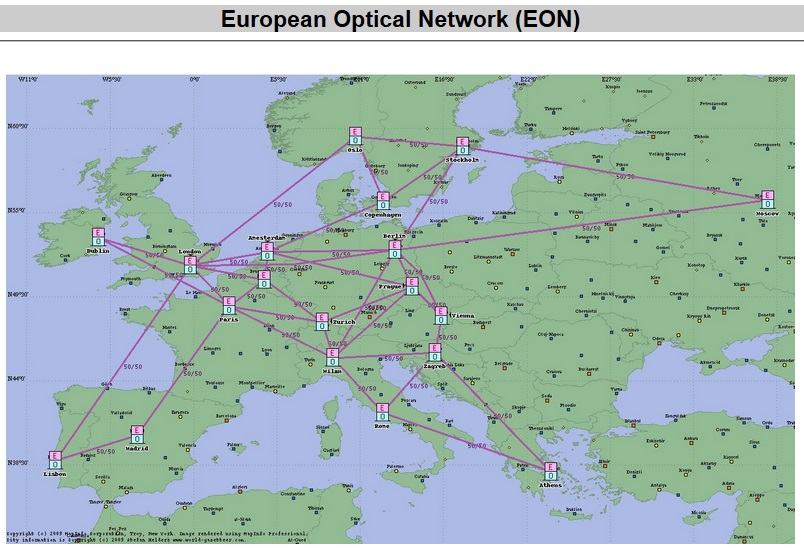
\includegraphics[width=\textwidth]{EON_Rede_Realista}
\caption{Physical topology of the realistic network.}
\end{figure}

Since the realistic network used in this case has already been mentioned previously in section \ref{Realistic_Network} we can assume that the table \ref{table_real_net} is the same and the table \ref{city_nodes_realnet} where each city contains a number of a node in the network also is the same.\\
The distance matrix constructed based on real distances between cities and the matrices of ODU's are also the same.
Finally, the total traffic for the two scenarios are:\\
Low Traffic: \textbf{2 TBits/s}; \quad High Traffic: \textbf{20 TBits/s};\\

\subsection{Dimensioning using ILP}
\begin{tcolorbox}	
\begin{tabular}{p{2.75cm} p{0.2cm} p{10.5cm}} 	
\textbf{Student Name}  &:& Tiago Esteves    (October 03, 2017 - )\\
\end{tabular}
\end{tcolorbox}

The initial subsection is the same as the subsection of the previous case so in this case it will be omitted presenting only the subsection of the results.
In this section we will do the dimensioning of the network mentioned in the previous section to calculate the value of your CAPEX, for this we will use the ILP model describe in section \ref{ILP_Opaque_Protection}.
This real network consists of many nodes and with many links between them as such the lpsolve takes immense time to get an optimal solution. Therefore, in this case, the execution time was defined as being two days (48 hours) and after that time presented the best solution.\\

\textbf{Scenario 1: Realistic Network Low Traffic} \label{Scenario3_opaque_p} \\

In this scenario we used the table \ref{table_real_net} and in the table \ref{result_ILP3} we can see the values calculated through MatLab and using the values indicated in table \ref{table_cost_opaque} we can finally calculate the CAPEX value.\\

Using equation \ref{linkCosts} : \\
$C_L$ = $($2 * 15 000 * 37$)$ + $($2 * 5 000 * 100 * 111 $)$ + $($24 * 4 000$)$ \\
$C_L$ = \textbf{112 206 000\euro} \\

Using equation \ref{electricalCostOpaque} : \\
$C_{exc}$ = $($19 * 10 000$)$ + 1 000 * $($4 000 + $($2 * 111 * 100$)$ $)$ \\
$C_N$ = $C_{exc}$ = \textbf{26 390 000 \euro} \\

$CAPEX$ = 112 206 000 + 26 390 000 = \textbf{138 596 000 \euro}\\

\begin{table}[h!]
\centering
\begin{tabular}{|| c | c||}
 \hline
 Number of optical channels & Value \\
 \hline\hline
in link (1,2) & 4 \\
in link (1,4) & 4 \\
in link (1,15) & 2 \\
in link (2,3) & 3 \\
in link (2,4) & 5 \\
in link (2,5) & 5 \\
in link (3,5) & 3 \\
in link (4,14) & 2 \\
in link (5,6) & 3 \\
in link (5,7) & 6 \\
in link (5,11) & 3 \\
in link (5,14) & 1 \\
in link (5,15) & 4 \\
in link (6,7) & 3 \\
in link (6,11) & 2 \\
in link (6,12) & 1 \\
in link (6,14) & 2 \\
in link (7,8) & 4 \\
in link (8,9) & 2 \\
in link (8,10) & 2 \\
in link (8,11) & 3 \\
in link (9,10) & 2 \\
in link (10,11) & 2 \\
in link (11,12) & 1 \\
in link (11,17) & 4 \\
in link (12,13) & 2 \\
in link (12,17) & 2 \\
in link (13,14) & 1 \\
in link (13,15) & 1 \\
in link (13,17) & 2 \\
in link (14,15) & 1 \\
in link (15,16) & 2 \\
in link (15,17) & 4 \\
in link (15,19) & 7 \\
in link (16,17) & 2 \\
in link (17,18) & 7 \\
in link (18,19) & 7 \\
\hline
\end{tabular}
\caption{Table with results}
\label{result_ILP3}
\end{table}

\textbf{Scenario 2: Realistic Network High Traffic} \label{Scenario4_opaque_p} \\

In this scenario we used again the table \ref{table_real_net} and in the table \ref{result_ILP4} we can see the values calculated through MatLab and using the values indicated in table \ref{table_cost_opaque} we can finally calculate the CAPEX value. \\

Using equation \ref{linkCosts} : \\
$C_L$ = $($2 * 15 000 * 37$)$ + $($2 * 5 000 * 100 * 1538$)$ + $($24 * 4 000$)$ \\
$C_L$ = \textbf{1 539 206 000 \euro} \\

Using equation \ref{electricalCostOpaque} : \\
$C_{exc}$ = $($19 * 10 000$)$ + 1 000 * $($40 000 + $($2 * 100 * 1538$)$ $)$ \\
$C_N$ = $C_{exc}$ = \textbf{347 790 000\euro} \\

$CAPEX$ = 1 539 206 000 + 347 790 000 = \textbf{1 886 996 000\euro}\\

\begin{table}[h!]
\centering
\begin{tabular}{|| c | c||}
 \hline
 Number of optical channels & Value \\
 \hline\hline
 in link (1,2) & 80 \\
in link (1,4) & 80 \\
in link (1,15) & 80 \\
in link (2,3) & 50 \\
in link (2,4) & 49 \\
in link (2,5) & 69 \\
in link (3,5) & 32 \\
in link (4,14) & 15 \\
in link (5,6) & 80 \\
in link (5,7) & 80 \\
in link (5,11) & 45 \\
in link (5,14) & 24 \\
in link (5,15) & 27 \\
in link (6,7) & 80 \\
in link (6,11) & 80 \\
in link (6,12) & 55 \\
in link (6,14) & 39 \\
in link (7,8) & 45 \\
in link (8,9) & 20 \\
in link (8,10) & 28 \\
in link (8,11) & 36 \\
in link (9,10) & 20 \\
in link (10,11) & 13 \\
in link (11,12) & 8 \\
in link (11,17) & 35 \\
in link (12,13) & 19 \\
in link (12,17) & 28 \\
in link (13,14) & 27 \\
in link (13,15) & 3 \\
in link (13,17) & 6 \\
in link (14,15) & 41 \\
in link (15,16) & 17 \\
in link (15,17) & 18 \\
in link (15,19) & 64 \\
in link (16,17) & 17 \\
in link (17,18) & 64 \\
in link (18,19) & 64 \\
\hline
\end{tabular}
\caption{Table with results}
\label{result_ILP4}
\end{table}


\subsection{Dimensioning using Heuristics}

\subsubsection{Heuristics Results}

\subsection{Comparative Analysis} 